\part{Down layer}
\label{down_layer}

Spodní vrstva se stará o spojení, jeho udržování, obnovování a fyzickou podobu přenášní dat. Je možné použít jeden ze dvou aplikačních protokolů (ve spodní vrstvě), a to HTTP(s) (viz \ref{down_layer.http}), nebo CRPP-binary (viz \ref{down_layer.crpp-binary}).

Spodní vrstva komunikuje s vrchní tím, že jí předává respektive dostává monolitické bloky dat. Tyto bloky jsou stejné na obou stranách spojení, viz diagram \ref{down_layer.pictures.monolithic_data_blocks}. Od okamžiku kdy bloky dat opustí vrstvu CRPP do jejich předání do této vrstvy na druhé straně spojení nesmí být změněno jejich pořadí (blok, který byl odeslán první, musí být jako první doručen). Může nastat situace, ve které je pořadí dat mezi protokoly spodní vrstvy jakkoli permutováno, ale mezi vrchními vrstvamy musí komunikace probíhat tak, jako by k žádnému prohození pořadí nedošlo.

\begin{figure}[h]
  \centering
  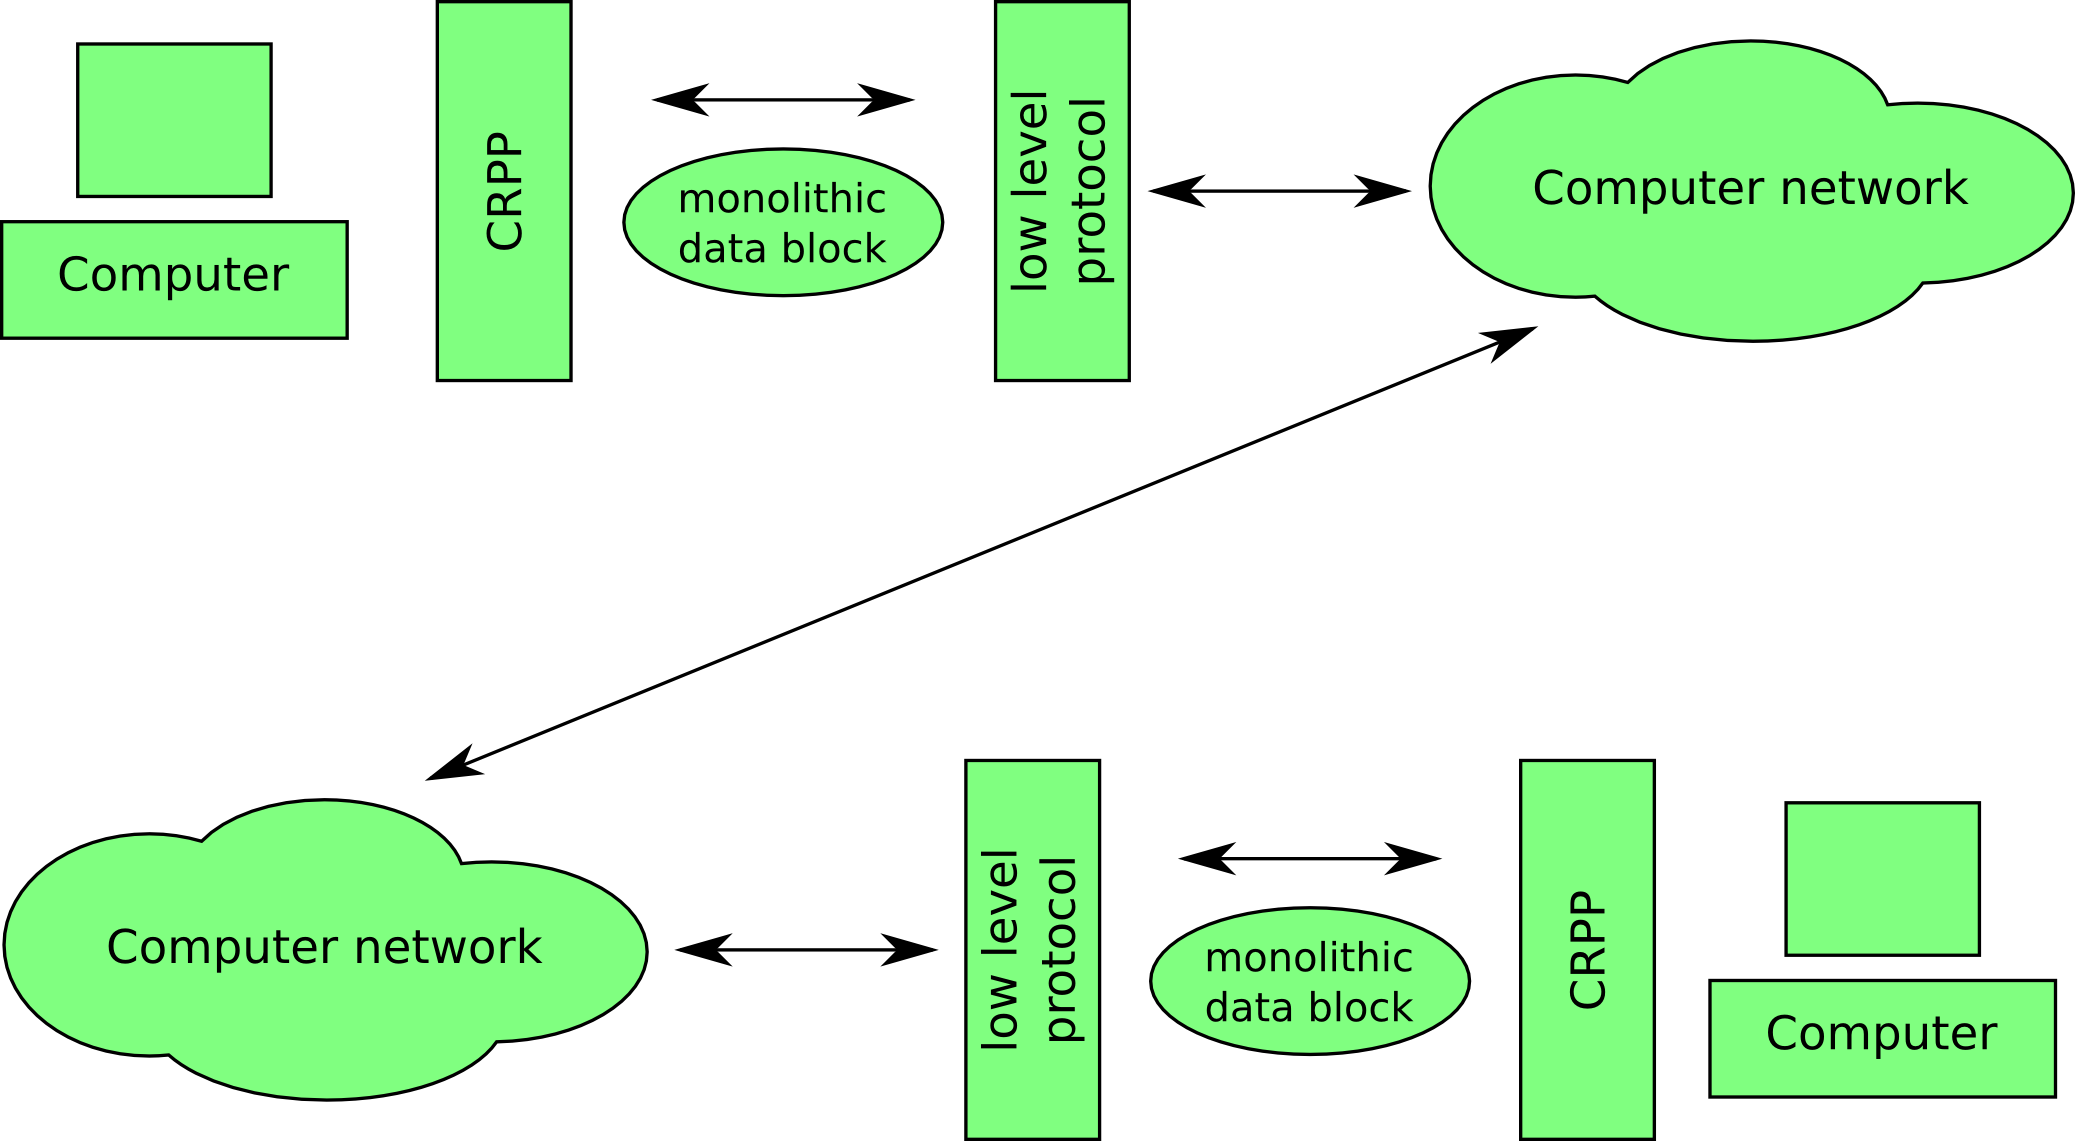
\includegraphics[width=0.80\textwidth]{diagrams/monolithic_data_blocks.png}
  \caption{Monolithic data blocks}
  \label{down_layer.pictures.monolithic_data_blocks}
\end{figure}

Veškerý úkol spodní vrstvy je brát posloupnosti bytů a ty doručovat na druhou stranu spojení ve stejním pořadí.

\chapter{CRPP-binary}
\label{down_layer.crpp-binary}

CRPP-binary je jednoduchý protokol, který umožnuje balit a odesílat data z vrchní vrstvy. Data z vrchní vrstvy se zabalí do packů a ty se na druhé straně opět rozbalují. Strukturu packu ilustruje obrázek \ref{down_layer.pictures.CRPP-binary}.

\begin{figure}[h]
  \centering
  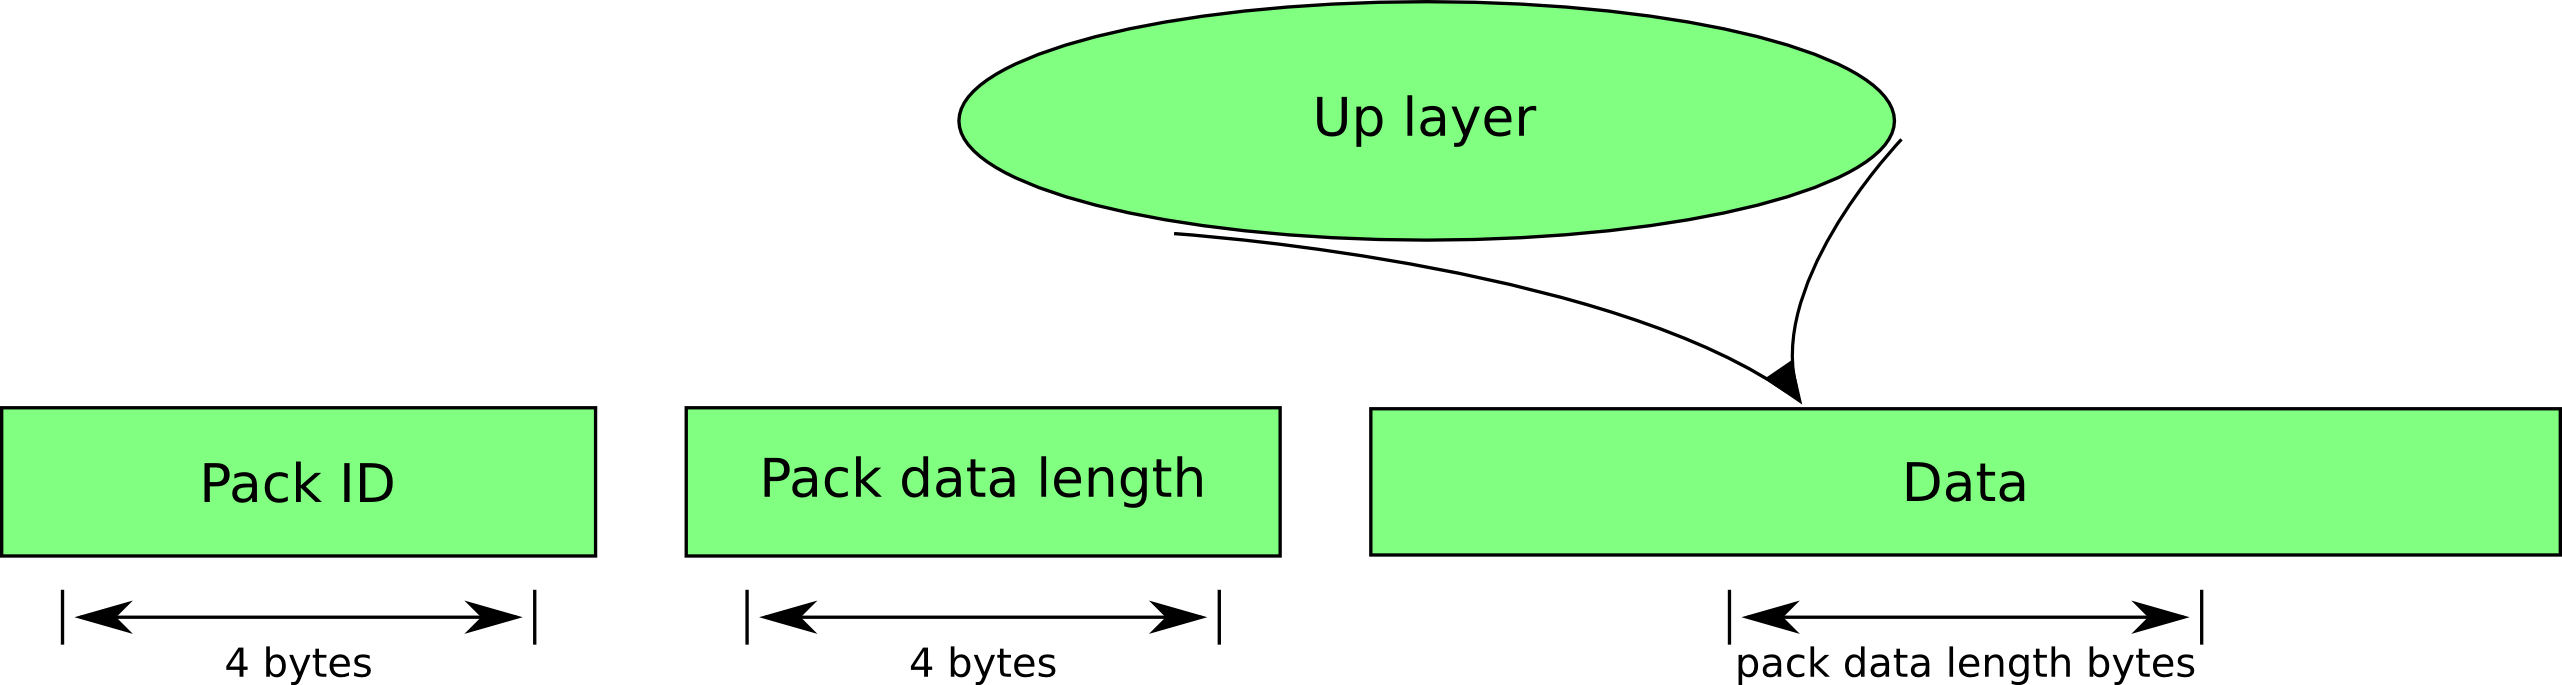
\includegraphics[width=0.80\textwidth]{diagrams/CRPP-binary.png}
  \caption{CRPP-binary pack}
  \label{down_layer.pictures.CRPP-binary}
\end{figure}

Pack se dělí na tři části, první dvě obsahuje hlavička packu a mají konstatní velikost. Třetí část obsahuje data packu. 

První čtyři byty packu obsahují ID packu, které by se mělo inkrementálně zvětšovat. ID je uvedeno jako bezznaménkové celé číslo, které je pospáno v části \ref{connection.data_types.unsigned_integer}.

Další čtyři byty (tedy pátý až osmý v pořadí) udávají celkovou délku přenášených dat bez hlavičky. Číslo je udáno opět podle specifikace v části \ref{connection.data_types.unsigned_integer}.

Zbytek zprávy jsou vlastní data, která zpracovává vrchní vrstva.

\chapter{HTTP(s)}
\label{down_layer.http}

% TODO: describe